Tunnistautumisessa on kolme osapuolta: asiakasohjelma, web-palvelu ja tunnistautumispalvelu \cite{nisti}. Osapuolet on esitetty kuvassa \ref{composition}, jossa on mukana myös tunnistautumispalvelun käyttämä käyttäjähallinta. Käyttäjähallinta voi olla myös osa tunnistautumispalvelua tai oma komponenttinsa. Tunnistautumisen kannalta sillä, onko käyttäjähallinta osa tunnistautumispalvelu vai erillinen komponentti, ei ole väliä.

\begin{figure}[ht]
\centering
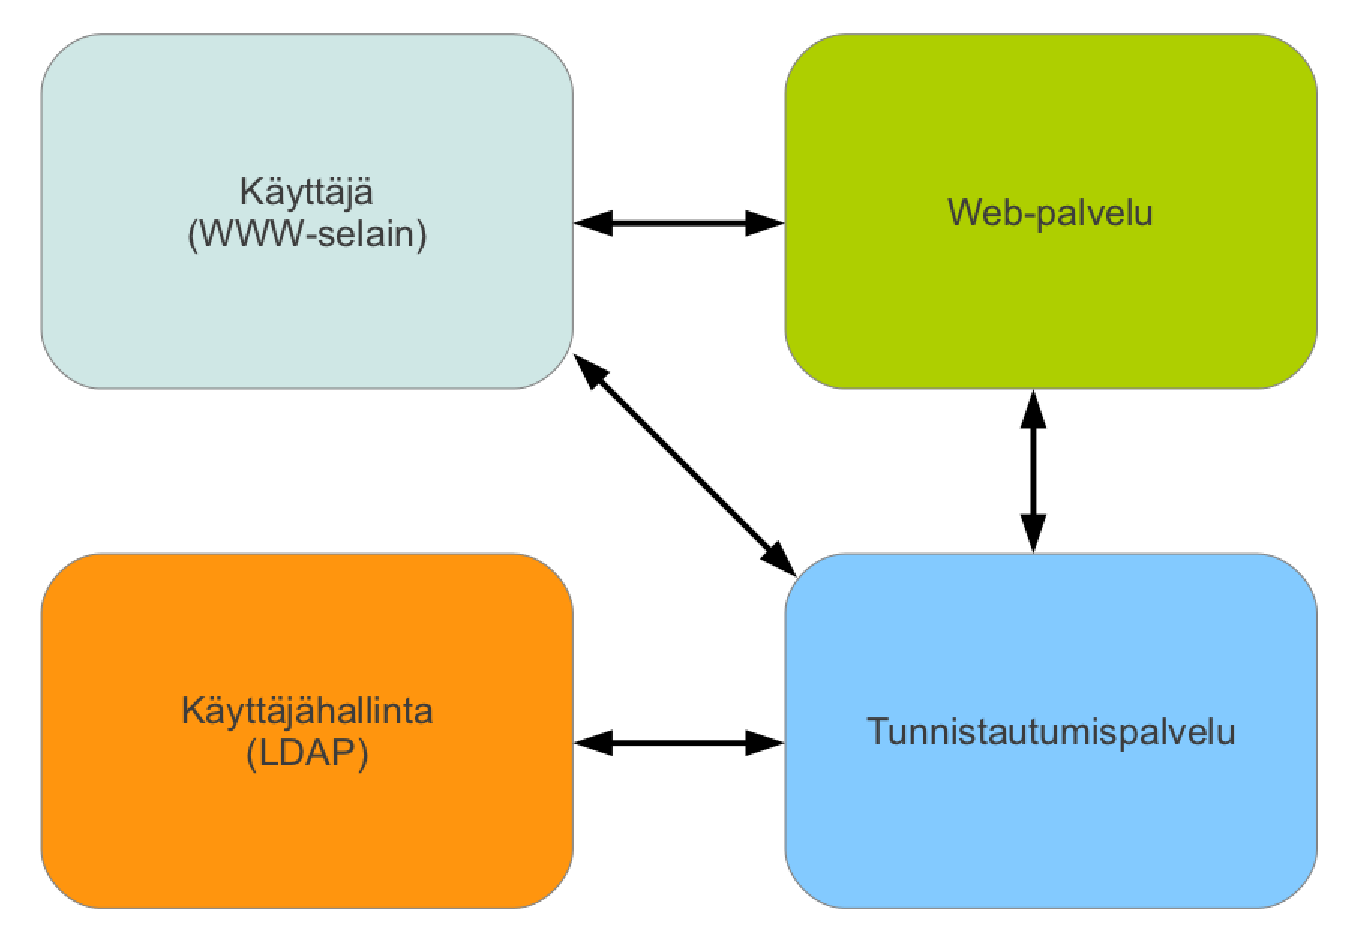
\includegraphics[width=0.7\textwidth]{teknologiat/composition.eps}
\caption{Keskitetyn tunnistautumisen osapuolet.}%
\label{composition}
\end{figure}

Ensimmäiseksi käyttäjä menee asiakasohjelmalla web-palveluun, joka pyytää tunnistautumista erillisessä tunnistautumispalvelussa. Käyttäjän asiakasohjelma ohjataan tunnistautumispalvelun sivulle, joka on yhteydessä organisaation käyttäjähallintaan. Käytetystä rajapintaprotokollasta riippuen käyttäjälle joko palautetaan todistus siitä, että hän on se jonka väittääkin olevansa tai avain, jonka avulla web-palvelu voi hakea käyttäjän tiedot tunnistautumispalvelulta.

Tunnistautumisprotokollia (kuten SAML, OpenID) käytettäessä käyttäjälle palautetaan valtuutustieto, joka on tunnistautumispalvelun allekirjoittama. Tämä valtuutustieto vahvistaa käyttäjän identiteetiksi sen, joka hän väittää olevansa \cite{nisti}.

Pääsynhallintaprotokollien (esim. OAuth) kohdalla käytetään ns. näennäistunnistautumista (pseudo authentication) \cite{distributed_web_security}. Tällöin web-palvelu voi hakea valtuutusavaimella käyttäjän tiedot tunnistautumispalvelusta. Käyttäjän identiteettiä ei siis suoraan varmenneta väitetyksi, mutta koska käyttäjällä on hallussaan avain, jolla pääsee hänen tietoihin käsiksi, oletetaan käyttäjän olevan se, jonka tiedot avaimella saadaan.

Useimmat tunnistautumisen vaiheet tapahtuvat käyttäjältä näkymättömissä selaimen uudelleenohjauksella. Käyttäjälle näkyvä vaihe on kirjautuminen tunnistautumispalvelulle, jolloin käyttäjältä pyydetään käyttäjätunnus ja salasana. Käyttäjän syötettä vaativat vaiheet on esitetty aiemmassa kuvassa \ref{facebook_login}.